\documentclass[a4paper]{article}



%Packages included
\usepackage{graphicx}
\usepackage{multicol}
\usepackage{hyperref}
\usepackage[headings]{fullpage}
\usepackage{fancyhdr}
\usepackage{float}
\usepackage{caption}
\usepackage{amsmath}
\usepackage{subcaption}
\usepackage[
backend=bibtex,
citestyle=authoryear,
sorting=none
]{biblatex}
\addbibresource{../bibliography/refrencedpapers.bib}

%set graphics path
\graphicspath{{../plotting/figures/}}

%opening
\title{The Effect of Bathymetry Changes on Meridional Overturning Currents}
\author{Marte Voorneveld\\
		5911591}


\pagestyle{fancy}
\fancyhead{}
\fancyfoot{}
\fancyhead[C]{\textit{The Effect of Bathymetry Changes on Overturning Circulation}}
\fancyhead[L]{\thepage}
\renewcommand{\headrulewidth}{0pt}

\begin{document}

\maketitle
\noindent\rule{\textwidth}{1pt}
\begin{abstract}

\end{abstract}
\noindent\rule{\textwidth}{1pt}
\begin{multicols}{2}
\section{Introduction}
The geometry and resulting bathymetry of our planet is an ever changing phenomenon. In the last 120 Ma the earth moved from having one major oceanic system in the Pacific with a single large continent to the current 3 ocean system (\cite{besse2002apparent}). The Bathymetry changes that occurred in this time period are characterized by the opening and closing of certain passages through which exchange of water between the oceanic basins is observed. The exact timing of passage openings is a topic of rigorous debate in literature (\cite{Scher2006Apr}, \cite{Schmidt2007Jan}).


One of the changes on which there is general consensus, is the inception and expansion of the Atlantic ocean and the resulting decrease in size of the Pacific basin. The creation of the Atlantic basin has had major effects on the earth's climate, especially resulting in massive localized changes such as the temperate European climate, due to the north Atlantic meridional overturning current (AMOC). This creates the current Northern sinking oceanic throughflow in the Atlantic. However it is unknown when exactly this northern sinking started. With the past non-existance of the Atlantic it must have started some time in the last 40Ma with the advent of a larger Atlantic (\cite{Abelson2017onset}). 

The result of these bathymetry changes on the oceanic stream function and the resulting overturning currents is something that has been previously studied by \cite{Mulder2017Jul}. They however found that using a Jacobian matrix for continuation in each of the model years fails to simulate the onset of the Northern sinking AMOC that is physically observed. Here we instead propose to use a general circulation ocean model with only a changing bathymetry keeping the same initial forcing for each time step. This eliminates the need for a continuation using the Jacobian matrix method proposed in \cite{Mulder2017Jul}.

This paper will focus solely on changes in bathymetry using simplified zonally averaged global forcings. The results of the model will be used to estimate global changes in oceanic through flow at the critical passages. Furthermore the strength of the meridional overturning currents (MOC) will be studied.


\section{Methods}



\subsection{Simplified Forcings}
The domain chosen is bounded by longitudes $\phi_E=-180^{\circ}$ and $\phi_W=-180^{\circ}$ and latitudes $\theta_N=80^{\circ}$ and $\theta_S=-80^{\circ}$ with periodic boundary conditions in the zonal direction.
Furthermore the model uses restoring boundary conditions first proposed by \cite{haney1971surface}. Restoring the boundary at the surface of the oceanic basin to be a certain value based of a forcing field for Sea Surface Temperature (SST), Sea Surface Salinity (SSS), and wind stresses ($\tau$).
 The depth profile has 15 layers with grid stretching. There are $90 \times 40$ grid points to make a $4^{\circ} \times 4^{\circ}$ resolution model. The forcings are prescribed as in \cite{Mulder2017Jul} by highly idealized zonally averaged forcings using current day values. The SST and Zonal wind stress are chosen as the analytical model in \cite{bryan1987parameter}. While SSS is chosen as a zonal average of current day values (from ECMWF but not sure how to cite). The meridional wind stress is set to zero. The maximum ocean depth is 5000m. The model also requires initial conditions for salinity and temperature, for this zonally averaged present day values are again used.

\end{multicols}
%example full width overturning

\begin{figure}[H]
\begin{subfigure}{.5\textwidth}
	\includegraphics[width=0.9\linewidth]{sss_sst_profile.png}
	\caption{SSS and SST}
	\label{fig:sst_sss}
\end{subfigure}
\begin{subfigure}{.5\textwidth}
	\centering
	% include first image
	\includegraphics[width=0.9\linewidth]{tau_x_profile.png}
	\caption{Zonal wind stress ($\tau_x$) profile}
	\label{fig:tau_X}
\end{subfigure}

\caption{Idealized forcing profiles}

\end{figure}

\begin{multicols}{2}
\subsection{Creating Bathymetries}
Creating the bathymetries for the model was done using bathymetries from Muller et al.\cite{Muller2008Mar} these were scaled to a 4 degree model and subsequently changed to address passage openings in the 4 degree case where, due to the low resolution of the model, choices have to be made with respect to the opening of certain passages. One of the choices that was made specifically is to change the bathymetry of the standard 4 degree model to a custom one made in the same process as the other bathymetries too more accurately portray changes that occur using this process. One of the choices that was made is that the northern Sea is closed of in all of the bathymetries. This is mainly due to the fact that 4 degree models do not have enough resolution to support This sea and can cause strange behaviour to occur. Also there is little connection to the other oceans, thus negating the need for such a basin to be in our model.

The main events that shape the oceanic passages can be devided into time periods. These time periods are defined as follows in this paper. This deviates from their definitions in literature but serves only as a means of applying a name to the time steps.

\begin{table}[H]
	\begin{tabular}{lll}
		&From &Until \\
		Paleocene & 65Ma&55Ma    \\
		Eocene    & 50Ma&35Ma     \\
		Oligocene & 30Ma&20Ma    \\
		Miocene   & 20Ma&Present 
	\end{tabular}
\end{table}

%TODO (Relevant figures from paleoscene showing changes)
The model is started in the Paleocene where in the beginning a vast Pacific exists almost serving as a single basin. This period is largely characterized by the growth and development of a larger atlantic basin. Serving to decrease the size of the pacific basin. This can be seen in Figure %TODO add figures showing diffirence in size. 
Where the changes during the paleoscene are shown.
\begin{figure}[H]
	
	
	\centering
	\begin{subfigure}[b]{\linewidth}
		\centering
		\includegraphics[width=\linewidth]{bathymetry/baath_65.png}
		\caption{Beginning of the Paleocene}
	\end{subfigure}
\begin{subfigure}[b]{\linewidth}
	\centering
	\includegraphics[width=\linewidth]{bathymetry/baath_50.png}
	\caption{End of the Paleocene}
\end{subfigure}
	\caption{}
	\label{fig:paleocene_bath}
\end{figure}


%TODO Eocene Drake-indian-tasman passages + depth

The Eocene in contrast to the Paleocene is destinguised by The opening of certain passages connecting oceanic basins. These effects are often studied extensively for each individual passage. Choosing the exact timespan for opening the passages is done manualy by looking at often active research takin into account big uncertaincies in the exact timing of the openings. The Eocene is characterized by several large events shown in Figure %todo add figure showing the events in detail
The first of such events that occurs is the indian continent colliding with the eurasian continent This has the effect of closing the deep water formations between the Thetys sea and the Indian ocean.
Next the Tasman passage is opened\cite{Lawver2003Sep} as a shallow passage slowly growing in size. The tasman passage opening is believed to have had a large impact on the onset of the ACC. The Total circulation of water around the antartic basin is finalized by the opening of the shallow Drake passage some 30Ma. 30Ma is specifically chosen to diffirentiate between the diffirent passage openings. Especially since there is still ongoing debate on the exact timing of drake passage opening.
%30ma drake passage opening (chosen as to diffirentiate between diffirent stages)
%35ma Indian passage closure
%35ma Tasman passage opening
%Indian continent colliding

%TODO Oligocene changes
The next time period is the oligocene Which is largely characterized by the deepening of the Tasman and drake passage and further expansion of the atlantic basin. It is believed %source
That the onset of the northern sinking atlantic started in this time period. Also the ACC probably is increasing in strenght.


%TODO Miocene

The miocene is Characterized by yet more increase in strenght of the ACC. Also Some more passage closures occur. Starting with the closure of the Thetys Seaway which had been decreasing in size in the previous 20Ma. Also the passage between modern day australia and indonesia is significantly decreasing in size due to the onset  of multiple vulcanic islands making the passage more narrow and shallow. Showing especially in this model. Further more the Thethys gateway
%0Ma current
%5Ma Wider Indonesia
%10ma last CAS
%14ma Thetys seaway last open 15ma first occurrence



Drake passage opening \cite{Scher2006Apr}

Tasman passage opening 

Central American seaway closure \cite{Molnar2008Jun} (deepwater 7Ma (10 for paper))\cite{Pindell1988Dec}

Tethys seaway closure \cite{Hamon2013Nov}

Widening of indonsian seaway (due to australia moving up.)


titis passage opening 

Choises made. 

Examples of where these choises interfere with reality.

Individual passages.

What age are we dealing with (Events/Changes observed in literature)


\end{multicols}
%example full width overturning
\begin{figure}[H]
	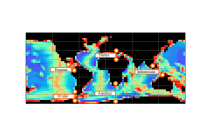
\includegraphics[width=\linewidth]{passages.png}
	\caption{Passages}
	\label{fig:passages}
\end{figure}
\begin{figure}[H]
	\includegraphics[width=\linewidth]{bathymetries_1.pdf}
\end{figure}
\begin{figure}[H]
	\includegraphics[width=\linewidth]{bathymetries_2.pdf}
	\caption{Bathymetries for each of the time steps studied in this model.}
	\label{fig:bathys}
\end{figure}

\begin{multicols}{2}




\subsection{Veros and Runtime}
\subsection{Veros}
Ocean modeling has been an area of continued progress. The resolutions of the models have been steadily increasing since the inception of the first computerized ocean models. However, due to the age of some of these models and the continued adaptation of often old legacy Fortran code, many models have become enormous hurdles to get started with often resulting in frustration. The Veros ocean model project is trying to tackle this problem with a totally new code base written entirely in Python (\cite{Hafner2018Aug}). 
Veros is an ocean general circulation model (GCM) based on the successful PyOm2 model. It was designed from the ground up with flexibility in mind. This flexibility cuts valuable time spent on figuring out the often cumbersome Fortran models of the past. Veros is specifically well suited for researching the effect of changes in both forcings and bathymetrys (depth profiles of the oceans). They can be easily edited using Python. These features in particular are heavily used in this paper. One of the most extensively used features for example is the fact that any bathymetry can, without further manual specifications, be used for stream function calculation.
The fact that it is fully written in Python is especially useful as python is far more widespread than Fortran and it is thus much easier to teach Veros to new students. 

In this case the models used in this paper are run on an 8 core (16 threads) machine using an MPI CPU configuration of 1 node. This is sufficient for the lower resolution models used in this paper. But Veros allows the usage of multiple nodes to do calculations on much higher resolution problems.



\section{Results}
\subsection{Stabilizing of the models}
(Section on when the integration was stopped. How good it is etc.)
$60/100$ done


\subsection{Passage throughflow}
\subsection{Passage throughflow}
As discussed in \fref{sec:throughflowp} the passage throughflow can be calculated using the velocity field for each time step. To do this a suitible location was chosen for each time step and passage such that there are no boundaries next to the passageways. This method is the same for each of the passages, noting that only zonal flow was studied. Thus we can study the effect of changes in bathymetry to on the relative strength of the flow.  The passageways have been labeled in figure (figure of these). The computed throughflow can be seen in \fref{fig:throughflow}. In this figure the onset of the ACC is clearly visible. Showing that due to the northward movement of Australia and the deepening of the drake passage the total volume transported by the ACC grows dramatically over time. Furthermore it can be seen that the closure of the drake passage causes the flow through the aghulas passage to reverse in direction. Furthermore, the throughflow through the panama passage is shown to slow due to both the onset of the ACC and the closure of the thetys seaway. Finally reversing the direction of flow through the panama passage at 15Ma due to the total closure of the thetys sea. The reversal of the Indonesian throughflow observed by \cite{Mulder2017Jul} is not observed with total throughflow always moving water east to west. This is however in agreement to the flow found by \cite{omta2003physical} in a shallow water model. Note however, that the land masks used by them are different to the land masks used in this paper.

\begin{figure}[H]
	\includegraphics[width=\linewidth]{throughflow}
	\caption{Total volume transport in Sverdups for 7 passages. Running from 65 milion years ago to the present day situation. Positive values indicate transport to the west}
	\label{fig:throughflow}
\end{figure}

Rather than looking only at volume transport in the upper layers the transport can also be split into a deep water transport layer ($<-2000m$) and a surface transport layer($>-2000m$). Doing this gives insight into the thermohaline circulation. In the deep water transport layer seen in \fref{fig:throughflow_bottom} we see a very diffirent picture to the total volume transport. It is however hard to draw any conclusions from this image. It is only 6 integration layers deep and fluctuations in the depth of each passage accounts for most of the differences comparing each time step.

(THIS NEEDS MORE SIMULATION TIME)
\begin{figure}[H]
	\includegraphics[width=\linewidth]{throughflow_deep_0_6}
	\caption{Total volume transport in the deep water layer ($<-2000m$) in Sverdups for 7 passages. Running from 65 milion years ago to the present day situation. Positive values indicate transport to the west}
	\label{fig:throughflow_bottom}
\end{figure}


To get an even better understanding of the flows, we can look at a vector field showing the direction of horizontal water displacement for each of the time steps. This is done by making a weighted mean of the horizontal flow field for each layer. Weighted by the volume of each grid cell. In this way each arrow actually represents relative flow velocity compared to other grid points. Thus showing the velocity field of the ocean. 

This field is shown in \fref{fig:flowfield}. Here the ACC is very noticible. The reversal of flow through the panama passage at $15Ma$ is the most interesting result here.  Where here we find the closure of the Thetys seaway to be the main factor. However, the reversal only occurs after the closure of the seaway. This is in contrast to the results obtained by \cite{omta2003physical} where the flow reversal was observed to coincide with the opening of the drake passage. Here we only observe a decease in volume transported through the passage, but no such reversal until the Thetys seaway is closed.

The largest changes in the flow field are observed in the Indian ocean. The indian continent moves northward at a very fast pace. After 55 Ma the flow through the passage north of the Indian continent is massively reduced and instead the water flows east of the continent into the thetys seaway. No "circum India" current is observed in any of the time steps. The position of the Indian continent does however seem to have a strong influence on the strength of the Aghulas sub-tropical gyre. This can probably be explained by the amount of water that is transported through the Tethys seaway. There being a large fluctuation in the strength of the gyre. The size of this gyre also increases with time due to this northward movement.


\subsection{Barotropic Stream function}
\subsection{Barotropic Stream function}
\label{sec:BSF}

Next we will look at the barotropic stream function for each of the time steps discussed in this paper. Some of the flows that are discussed in this section are closely related to the flows explained in \cref{sec:throughflow}. Here we will have a stronger focus on the gyres seen in the ocean and their relative strength in a time sense. Each of the oceanic basins is discussed in detail. An overview of each of the barotropic stream functions can be seen in \cref{fig:bsf_total}. The boundary values of the BSF are not shown here. This is due to the previously stated fact that they are excluded from the model output produced by Veros. It must however be noted that this does not mean that flows through the passages are not modeled. In this case the barotropic stream function serves only to see the major ocean gyres and how water is transported in these gyres.

\subsubsection{Indian Ocean}
The Indian ocean and especially the indian Continent moving northward seems to be one of the most interesting artifacts of these simulations. When the Indian continent is still within the subtropical gyre range in the early Paleocene. We see that it has a large blocking effect on the Subtropical gyre in the Indian ocean. We also see, as observed in the Flow patterns for each of the basins, a change from current moving north over india to moving east and then up towards the Atlantic basin. Something that is simmilarly observed in \cite{omta2003physical}. However as noted in \cref{sec:throughflowp} we do not observe a the often shown circum-India current (\cite{omta2003physical};
\cite{von2006effect}). In the Paleocene the Indian continent seems to be the most influential in establishing the ocean gyres. The stark contrast between 65 and 60Ma BSF can be explained due to the island ridge north of India.
\subsubsection{Pacific Ocean}
The pacific ocean is of particular interest in this case. One of the main things that we see is a large fluctuation in the strength of the southern subtropical gyre. This fluctuation is a diffirence of $\pm 20 Sv$.  Especially when the ACC is not yet developed. This is especially visible in the Paleocene and early Eocene where the transport is particularly extreme at places where the Thetys throughflow is the largest. The size of the southern subtropical gyre seems to relate to the Thetys values seen in \prettyref{fig:throughflow}. Here we see a round earth current through the Thetys, Indonesian and Panama passages exists. This can explain why such a largely positive streamfunction can be seen in the southern pacific. This  Where this only changes with the onset of the ACC.
\subsubsection{Atlantic Ocean}
The Atlantic basin seems to be the most quiet basin here. This is in large part thanks to the fact that the atlantic basin is so small in the beginning of our time series. One of the flows that is of particular interest here is the subpolar gyre that exists the entire time until the onset of the ACC where it is replaced. The onset of the ACC also seems to coincide with the growth of the southern subtropical gyre. Also the northern subpolar gyre is hardly visible here at all. This is likely due to low resolution used by this model not being able to have proper in and outflow of the arctic sea here. 


%The detachment of Australia to the antarctic current at 35Ma introduces a strong flow ($17Sv$) through the newly formed Tasman passage. However there is no

\subsection{MOC Stream function}
Section on the meridional overturning current



\section{Summary}
%\section{Summary}
In this paper we have presented a simplified approach to the modeling of past climate systems using Veros. This paper focused heavily on simplified forcings of the global oceanic basins. This allows in contrast to past attempts using continuation approaches to be able to efficiently look at the effect of changes in geometry on the major oceanic flows. The results shown here are of relatively low resolution and highly idealized boundary conditions. But they still manage to capture many of the effects seen in more complex coupled models. The integrations were done on a consumer computer showing that it is now possible to do big ocean simulation research on readily availible hardware.

The analysis of the results focused specifically on the multiple passage changes that occured in the time period. Specifically noting the effects on the thermohaline circulation.


$0/100$ done

\section{Discussion}
The method presented here for an alternative to the continuation approach suggested by \cite{Mulder2017Jul} still has quite a few problems. First of all, the $4^{\circ}$ resolution together with the limited number of depth layers is one of the main problems. The limited depth layers fail to accurately capture even the present day overturning circulation. Here we note that the same can be said for a model with present day forcings as noted in \cref{sec:mocQual}.

The possibility of using a 1 or 2 degree Veros model for this paper was extensively explored. But issues often arose with the exact values of constants and frequent invalid value errors to do with eddy kinetic energy could not be fixed in time for this paper.

The 4 degree model also took quite a bit of time to be adapted for the customized forcings and bathymetries. This is due to the fact that the method for determining boundary conditions for islands would often find more islands than exist in the model. Resulting in having to customize each setup individually for its bathymetry to accept the islands present. This is also why $180^{\circ} E$ was used as the boundary longitude instead of the default $0^{\circ}$. These problems are one of the main driving forces behind the decision to limit the integration time to just 500 years. A better estimate for the overturning circulation can probably be made already when extending the integration time to 1000 years

Another major change that is neglected in this paper is the total absence of change in surface forcings over time. Even though it is known that these change drastically even in short time spans. We also have some general knowledge of global average temperature for the time period discussed here. However the search for a dataset for each time step has proven futile. Often large uncertainties exist which would result in much more confusing results. This left us with the decision to not bother with any changes in the forcings.

A lot of future research is possible in the topic of oceanic throughflow. More accurate bathymetries are being produced due to breakthroughs in geological techniques (\cite{Baatsen2016Aug}). These, coupled with a higher resolution model will probably result in even more accurate depictions of the past oceanic systems. Research on this topic is of particular importance because of the present day observed changes in strength of the MOC and to enhance the feedback loop between what is observed in geological excavations and models of our planet.
$0/100$ done


%\section{Test images}
%\begin{figure}[H]
%	\includegraphics[width=\linewidth]{overturning_overview.png}
%	\caption{test caption}
%	\label{fig:example1}
%\end{figure}
%\end{multicols}
%%example full width overturning
%\begin{figure}[H]
%	\includegraphics[width=\linewidth]{overturning_overview.png}
%	\caption{test caption}
%	\label{fig:example1}
%\end{figure}
%
%\begin{multicols}{2}

\printbibliography

\end{multicols}



\end{document}
